% Options for packages loaded elsewhere
\PassOptionsToPackage{unicode}{hyperref}
\PassOptionsToPackage{hyphens}{url}
%
\documentclass[
]{article}
\usepackage{amsmath,amssymb}
\usepackage{iftex}
\ifPDFTeX
  \usepackage[T1]{fontenc}
  \usepackage[utf8]{inputenc}
  \usepackage{textcomp} % provide euro and other symbols
\else % if luatex or xetex
  \usepackage{unicode-math} % this also loads fontspec
  \defaultfontfeatures{Scale=MatchLowercase}
  \defaultfontfeatures[\rmfamily]{Ligatures=TeX,Scale=1}
\fi
\usepackage{lmodern}
\ifPDFTeX\else
  % xetex/luatex font selection
\fi
% Use upquote if available, for straight quotes in verbatim environments
\IfFileExists{upquote.sty}{\usepackage{upquote}}{}
\IfFileExists{microtype.sty}{% use microtype if available
  \usepackage[]{microtype}
  \UseMicrotypeSet[protrusion]{basicmath} % disable protrusion for tt fonts
}{}
\makeatletter
\@ifundefined{KOMAClassName}{% if non-KOMA class
  \IfFileExists{parskip.sty}{%
    \usepackage{parskip}
  }{% else
    \setlength{\parindent}{0pt}
    \setlength{\parskip}{6pt plus 2pt minus 1pt}}
}{% if KOMA class
  \KOMAoptions{parskip=half}}
\makeatother
\usepackage{xcolor}
\usepackage[margin=1in]{geometry}
\usepackage{color}
\usepackage{fancyvrb}
\newcommand{\VerbBar}{|}
\newcommand{\VERB}{\Verb[commandchars=\\\{\}]}
\DefineVerbatimEnvironment{Highlighting}{Verbatim}{commandchars=\\\{\}}
% Add ',fontsize=\small' for more characters per line
\usepackage{framed}
\definecolor{shadecolor}{RGB}{248,248,248}
\newenvironment{Shaded}{\begin{snugshade}}{\end{snugshade}}
\newcommand{\AlertTok}[1]{\textcolor[rgb]{0.94,0.16,0.16}{#1}}
\newcommand{\AnnotationTok}[1]{\textcolor[rgb]{0.56,0.35,0.01}{\textbf{\textit{#1}}}}
\newcommand{\AttributeTok}[1]{\textcolor[rgb]{0.13,0.29,0.53}{#1}}
\newcommand{\BaseNTok}[1]{\textcolor[rgb]{0.00,0.00,0.81}{#1}}
\newcommand{\BuiltInTok}[1]{#1}
\newcommand{\CharTok}[1]{\textcolor[rgb]{0.31,0.60,0.02}{#1}}
\newcommand{\CommentTok}[1]{\textcolor[rgb]{0.56,0.35,0.01}{\textit{#1}}}
\newcommand{\CommentVarTok}[1]{\textcolor[rgb]{0.56,0.35,0.01}{\textbf{\textit{#1}}}}
\newcommand{\ConstantTok}[1]{\textcolor[rgb]{0.56,0.35,0.01}{#1}}
\newcommand{\ControlFlowTok}[1]{\textcolor[rgb]{0.13,0.29,0.53}{\textbf{#1}}}
\newcommand{\DataTypeTok}[1]{\textcolor[rgb]{0.13,0.29,0.53}{#1}}
\newcommand{\DecValTok}[1]{\textcolor[rgb]{0.00,0.00,0.81}{#1}}
\newcommand{\DocumentationTok}[1]{\textcolor[rgb]{0.56,0.35,0.01}{\textbf{\textit{#1}}}}
\newcommand{\ErrorTok}[1]{\textcolor[rgb]{0.64,0.00,0.00}{\textbf{#1}}}
\newcommand{\ExtensionTok}[1]{#1}
\newcommand{\FloatTok}[1]{\textcolor[rgb]{0.00,0.00,0.81}{#1}}
\newcommand{\FunctionTok}[1]{\textcolor[rgb]{0.13,0.29,0.53}{\textbf{#1}}}
\newcommand{\ImportTok}[1]{#1}
\newcommand{\InformationTok}[1]{\textcolor[rgb]{0.56,0.35,0.01}{\textbf{\textit{#1}}}}
\newcommand{\KeywordTok}[1]{\textcolor[rgb]{0.13,0.29,0.53}{\textbf{#1}}}
\newcommand{\NormalTok}[1]{#1}
\newcommand{\OperatorTok}[1]{\textcolor[rgb]{0.81,0.36,0.00}{\textbf{#1}}}
\newcommand{\OtherTok}[1]{\textcolor[rgb]{0.56,0.35,0.01}{#1}}
\newcommand{\PreprocessorTok}[1]{\textcolor[rgb]{0.56,0.35,0.01}{\textit{#1}}}
\newcommand{\RegionMarkerTok}[1]{#1}
\newcommand{\SpecialCharTok}[1]{\textcolor[rgb]{0.81,0.36,0.00}{\textbf{#1}}}
\newcommand{\SpecialStringTok}[1]{\textcolor[rgb]{0.31,0.60,0.02}{#1}}
\newcommand{\StringTok}[1]{\textcolor[rgb]{0.31,0.60,0.02}{#1}}
\newcommand{\VariableTok}[1]{\textcolor[rgb]{0.00,0.00,0.00}{#1}}
\newcommand{\VerbatimStringTok}[1]{\textcolor[rgb]{0.31,0.60,0.02}{#1}}
\newcommand{\WarningTok}[1]{\textcolor[rgb]{0.56,0.35,0.01}{\textbf{\textit{#1}}}}
\usepackage{longtable,booktabs,array}
\usepackage{calc} % for calculating minipage widths
% Correct order of tables after \paragraph or \subparagraph
\usepackage{etoolbox}
\makeatletter
\patchcmd\longtable{\par}{\if@noskipsec\mbox{}\fi\par}{}{}
\makeatother
% Allow footnotes in longtable head/foot
\IfFileExists{footnotehyper.sty}{\usepackage{footnotehyper}}{\usepackage{footnote}}
\makesavenoteenv{longtable}
\usepackage{graphicx}
\makeatletter
\def\maxwidth{\ifdim\Gin@nat@width>\linewidth\linewidth\else\Gin@nat@width\fi}
\def\maxheight{\ifdim\Gin@nat@height>\textheight\textheight\else\Gin@nat@height\fi}
\makeatother
% Scale images if necessary, so that they will not overflow the page
% margins by default, and it is still possible to overwrite the defaults
% using explicit options in \includegraphics[width, height, ...]{}
\setkeys{Gin}{width=\maxwidth,height=\maxheight,keepaspectratio}
% Set default figure placement to htbp
\makeatletter
\def\fps@figure{htbp}
\makeatother
\setlength{\emergencystretch}{3em} % prevent overfull lines
\providecommand{\tightlist}{%
  \setlength{\itemsep}{0pt}\setlength{\parskip}{0pt}}
\setcounter{secnumdepth}{-\maxdimen} % remove section numbering
\usepackage{pdfpages}
\usepackage{graphicx}
\ifLuaTeX
  \usepackage{selnolig}  % disable illegal ligatures
\fi
\IfFileExists{bookmark.sty}{\usepackage{bookmark}}{\usepackage{hyperref}}
\IfFileExists{xurl.sty}{\usepackage{xurl}}{} % add URL line breaks if available
\urlstyle{same}
\hypersetup{
  hidelinks,
  pdfcreator={LaTeX via pandoc}}

\author{}
\date{\vspace{-2.5em}}

\begin{document}


\includepdf{page_de_garde.pdf}

\thispagestyle{empty}
\newpage

\setcounter{tocdepth}{4}                
\renewcommand{\contentsname}{\textcolor{blue}{Sommaire}}

\textcolor{blue}{\tableofcontents} \newpage

\hypertarget{partie-i}{%
\section{PARTIE I}\label{partie-i}}

\hypertarget{pruxe9paration-des-donnuxe9es}{%
\subsection{1.Préparation des
données}\label{pruxe9paration-des-donnuxe9es}}

\hypertarget{description}{%
\subsubsection{1.1 Description}\label{description}}

Dans cette sous partie aucune n'instruction n'a été demandée.Elle a été
faite afin de permettre à l'élève de mieux se familiariser avec la base
Base\_Partie 1 qui: regroupe les variables relatives à certains
caractéristiques socio-professionnels des dirigeants des différents PME,
les coordonnées géographique des PME et la date de soumission des
informations de la PME à l'enqueteur. La résolution des questions
suivantes se fera essentiellement à l'aide de ces données.

\hypertarget{importation-et-mise-en-forme}{%
\subsubsection{1.2 importation et mise en
forme}\label{importation-et-mise-en-forme}}

dans section il s'agira de faire quelques opérations sur la base de
donnée Base\_partie 1 à savoir l'importation des données et la détection
des valeurs manquantes par variable.

\hypertarget{importation-de-la-base-de-donnuxe9}{%
\paragraph{1.2.1 importation de la base de
donné}\label{importation-de-la-base-de-donnuxe9}}

\begin{Shaded}
\begin{Highlighting}[]
\NormalTok{projet}\OtherTok{\textless{}{-}} \FunctionTok{read\_excel}\NormalTok{(}\StringTok{"Base\_Partie 1.xlsx"}\NormalTok{,}
                    \AttributeTok{range=}\ConstantTok{NULL}\NormalTok{,}
                    \AttributeTok{col\_names =} \ConstantTok{TRUE}\NormalTok{,}
                    \AttributeTok{col\_types =} \ConstantTok{NULL}\NormalTok{,}
\NormalTok{                    ) }\CommentTok{\#la base de donnée étant sous l\textquotesingle{}extension xlsx,}
\CommentTok{\#la fonction read\_excel du package readxl est la mieux adapter pour son importation.}
\end{Highlighting}
\end{Shaded}

\hypertarget{faisons-un-tableau-ruxe9sumant-les-valeurs-manquantes-par-valeur}{%
\paragraph{1.2.2 faisons un tableau résumant les valeurs manquantes par
valeur}\label{faisons-un-tableau-ruxe9sumant-les-valeurs-manquantes-par-valeur}}

pour le faire nous ferons usage de la fonction miss\_var\_summary du
package naniar qui à pour role principal de ressortir un résumé des
valeurs manquantes pour chaque variables de la base de donnée. En effet,
elle permet de calculer pour chaque variable le nombre total des valeurs
manquantes ainsi que la proportion de valeur manquante pour chaque
variable.

\begin{Shaded}
\begin{Highlighting}[]
\NormalTok{data\_miss}\OtherTok{=}\FunctionTok{miss\_var\_summary}\NormalTok{(projet)}
\FunctionTok{kable}\NormalTok{(}\FunctionTok{head}\NormalTok{(data\_miss))}
\end{Highlighting}
\end{Shaded}

\begin{longtable}[]{@{}lrr@{}}
\toprule\noalign{}
variable & n\_miss & pct\_miss \\
\midrule\noalign{}
\endhead
\bottomrule\noalign{}
\endlastfoot
q17 & 131 & 52.4 \\
q19 & 120 & 48.0 \\
q14b & 1 & 0.4 \\
q16 & 1 & 0.4 \\
key & 0 & 0.0 \\
q1 & 0 & 0.0 \\
\end{longtable}

\hypertarget{vuxe9rifions-sil-y-a-des-valeurs-manquantes-pour-la-variable-key-dans-la-base-projet.-si-oui-identifier-la-ou-les-pme-concernuxe9es.}{%
\paragraph{1.2.3 Vérifions s'il y a des valeurs manquantes pour la
variable key dans la base projet. Si oui, identifier la (ou les) PME
concernée(s).}\label{vuxe9rifions-sil-y-a-des-valeurs-manquantes-pour-la-variable-key-dans-la-base-projet.-si-oui-identifier-la-ou-les-pme-concernuxe9es.}}

pour la résolution de cette question nous avons fait usage à une
structure conditionnelle qui retournera si la variable key contient ou
non des valeurs manquantes et comme après éxécution du code key n'a pas
de valeur manquantes, aucune PME ne sera identifiée.

\begin{Shaded}
\begin{Highlighting}[]
\NormalTok{has\_missing }\OtherTok{\textless{}{-}} \FunctionTok{any}\NormalTok{(}\FunctionTok{is.na}\NormalTok{(projet}\SpecialCharTok{$}\NormalTok{key))}\CommentTok{\# vérifie si la variable key contient des valeurs NA}
\CommentTok{\# Affichage du résultat}
\ControlFlowTok{if}\NormalTok{ (has\_missing) \{}
  \FunctionTok{print}\NormalTok{(}\StringTok{"Il y a des valeurs manquantes pour la variable \textquotesingle{}key\textquotesingle{}."}\NormalTok{)}
\NormalTok{\} }\ControlFlowTok{else}\NormalTok{ \{}
  \FunctionTok{print}\NormalTok{(}\StringTok{"Il n\textquotesingle{}y a pas de valeur manquante pour la variable \textquotesingle{}key\textquotesingle{}."}\NormalTok{)}
\NormalTok{\}}
\end{Highlighting}
\end{Shaded}

\begin{verbatim}
## [1] "Il n'y a pas de valeur manquante pour la variable 'key'."
\end{verbatim}

\hypertarget{cruxe9ation-de-variables}{%
\subsubsection{1.3 Création de
variables}\label{cruxe9ation-de-variables}}

\hypertarget{renomons-les-variables-q1q2-et-q23-respectivement-en-ruxe9gionduxe9partement-et-sexe}{%
\paragraph{1.3.1 Renomons les variables q1,q2 et q23 respectivement en
région,département et
sexe}\label{renomons-les-variables-q1q2-et-q23-respectivement-en-ruxe9gionduxe9partement-et-sexe}}

pour cela nous ferons juste usage de la fonction renames de
\textbf{dplyr}

\begin{Shaded}
\begin{Highlighting}[]
\NormalTok{projet}\OtherTok{\textless{}{-}}\NormalTok{ projet }\SpecialCharTok{\%\textgreater{}\%}\NormalTok{ dplyr}\SpecialCharTok{::}\FunctionTok{rename}\NormalTok{(}\AttributeTok{region=}\NormalTok{ q1, }\AttributeTok{departement=}\NormalTok{q2, }\AttributeTok{sexe=}\NormalTok{q23) }\CommentTok{\#"\%\textgreater{}\%" permet de chaîner des opérations de transformation de données en passant le résultat d\textquotesingle{}une étape à la suivante.}
\end{Highlighting}
\end{Shaded}

\hypertarget{cruxe9ons-la-variable-sexe_2-qui-vaut-1-si-sexe-uxe9gale-uxe0-femme-et-0-sinon}{%
\paragraph{1.3.2 Créons la variable sexe\_2 qui vaut 1 si sexe égale à
femme et 0
sinon}\label{cruxe9ons-la-variable-sexe_2-qui-vaut-1-si-sexe-uxe9gale-uxe0-femme-et-0-sinon}}

Pour ceci nous ferrons juste usage des fonctions mutate et if\_else du
package dplyr.

\begin{Shaded}
\begin{Highlighting}[]
\NormalTok{projet }\OtherTok{\textless{}{-}}\NormalTok{ projet }\SpecialCharTok{\%\textgreater{}\%}
  \CommentTok{\# Mutate permet l\textquotesingle{}ajout de la colonne sexe\_2 au data frame projet}
  \FunctionTok{mutate}\NormalTok{(}\AttributeTok{sexe\_2 =} \FunctionTok{if\_else}\NormalTok{(sexe}\SpecialCharTok{==}\StringTok{"Femme"}\NormalTok{,}\DecValTok{1}\NormalTok{,}\DecValTok{0}\NormalTok{))}
\end{Highlighting}
\end{Shaded}

\hypertarget{cruxe9ons-un-data-frame-nommer-langue-qui-prend-la-variable-key-et-les-variables-correspondantes-aux-langues-parluxe9es.}{%
\paragraph{1.3.3 Créons un data frame nommer langue qui prend la
variable key et les variables correspondantes aux langues
parlées.}\label{cruxe9ons-un-data-frame-nommer-langue-qui-prend-la-variable-key-et-les-variables-correspondantes-aux-langues-parluxe9es.}}

pour le faire nous ferons usage de la fonction select de dplyr. Comme
les variables correspondantes aux langues parlées commence tous par
\textbf{q24a\_} , l'usage de \textbf{starts\_with} sera très bénéfique
car il permettra de selectionner aisement toutes les variables de la
base qui commencent par \textbf{q25a\_} dont toutes les langues parlées
présentes dans la base.

\begin{Shaded}
\begin{Highlighting}[]
\NormalTok{langues}\OtherTok{\textless{}{-}}\NormalTok{projet }\SpecialCharTok{\%\textgreater{}\%}\NormalTok{ dplyr}\SpecialCharTok{::}\FunctionTok{select}\NormalTok{(key,}\FunctionTok{starts\_with}\NormalTok{(}\StringTok{"q24a\_"}\NormalTok{))}
\end{Highlighting}
\end{Shaded}

\hypertarget{analyses-descriptives}{%
\subsection{ANALYSES DESCRIPTIVES}\label{analyses-descriptives}}

Déterminons la répartion des PME suivant le sexe, le niveau
d'instrution,le statut juridique,le propriétaire/locataire, le statut
juridique et le sexe, le niveau d'inscrution et le sexe, propriétaire ou
locataire et le sexe.

pour cela nous créerons deux tableaux distinct que nous rélierons par la
suite avec la fonction ** ** nous allons reliés les deux tableaux.

\begin{Shaded}
\begin{Highlighting}[]
\NormalTok{projet}\SpecialCharTok{\%\textgreater{}\%} 
\NormalTok{  dplyr}\SpecialCharTok{::}\FunctionTok{select}\NormalTok{(sexe,q25,q12,q81)}\SpecialCharTok{\%\textgreater{}\%}
\NormalTok{  gtsummary}\SpecialCharTok{::}\FunctionTok{tbl\_summary}\NormalTok{(}
    \AttributeTok{by=}\NormalTok{sexe,}
    \AttributeTok{label=}\FunctionTok{list}\NormalTok{(q25}\SpecialCharTok{\textasciitilde{}}\StringTok{"Niveau d\textquotesingle{}instruction"}\NormalTok{, }
\NormalTok{               q12}\SpecialCharTok{\textasciitilde{}}\StringTok{"statut Juridique"}\NormalTok{,}
\NormalTok{               q81}\SpecialCharTok{\textasciitilde{}}\StringTok{"propriétaire/locataire"}
\NormalTok{    ),}
   \AttributeTok{statistic =} \FunctionTok{list}\NormalTok{(}\FunctionTok{all\_categorical}\NormalTok{()}\SpecialCharTok{\textasciitilde{}} \StringTok{"\{n\}\%"}\NormalTok{),}
   \AttributeTok{missing=}\StringTok{"always"}\NormalTok{,}
   \AttributeTok{missing\_text=}\StringTok{"Missing"}\NormalTok{,}
   \AttributeTok{percent=}\StringTok{"column"}
   
\NormalTok{  )}\SpecialCharTok{\%\textgreater{}\%}
\FunctionTok{add\_overall}\NormalTok{()}\SpecialCharTok{\%\textgreater{}\%}
\FunctionTok{bold\_labels}\NormalTok{()}
\end{Highlighting}
\end{Shaded}

\begin{verbatim}
## Table printed with `knitr::kable()`, not {gt}. Learn why at
## https://www.danieldsjoberg.com/gtsummary/articles/rmarkdown.html
## To suppress this message, include `message = FALSE` in code chunk header.
\end{verbatim}

\begin{longtable}[]{@{}
  >{\raggedright\arraybackslash}p{(\columnwidth - 6\tabcolsep) * \real{0.3068}}
  >{\centering\arraybackslash}p{(\columnwidth - 6\tabcolsep) * \real{0.2500}}
  >{\centering\arraybackslash}p{(\columnwidth - 6\tabcolsep) * \real{0.2273}}
  >{\centering\arraybackslash}p{(\columnwidth - 6\tabcolsep) * \real{0.2159}}@{}}
\toprule\noalign{}
\begin{minipage}[b]{\linewidth}\raggedright
\textbf{Characteristic}
\end{minipage} & \begin{minipage}[b]{\linewidth}\centering
\textbf{Overall}, N = 250
\end{minipage} & \begin{minipage}[b]{\linewidth}\centering
\textbf{Femme}, N = 191
\end{minipage} & \begin{minipage}[b]{\linewidth}\centering
\textbf{Homme}, N = 59
\end{minipage} \\
\midrule\noalign{}
\endhead
\bottomrule\noalign{}
\endlastfoot
\textbf{Niveau d'instruction} & & & \\
Aucun niveau & 79\% & 70\% & 9\% \\
Niveau primaire & 56\% & 48\% & 8\% \\
Niveau secondaire & 74\% & 56\% & 18\% \\
Niveau Superieur & 41\% & 17\% & 24\% \\
Missing & 0 & 0 & 0 \\
\textbf{statut Juridique} & & & \\
Association & 6\% & 3\% & 3\% \\
GIE & 179\% & 149\% & 30\% \\
Informel & 38\% & 32\% & 6\% \\
SA & 7\% & 1\% & 6\% \\
SARL & 13\% & 2\% & 11\% \\
SUARL & 7\% & 4\% & 3\% \\
Missing & 0 & 0 & 0 \\
\textbf{propriétaire/locataire} & & & \\
Locataire & 24\% & 16\% & 8\% \\
Propriétaire & 226\% & 175\% & 51\% \\
Missing & 0 & 0 & 0 \\
\end{longtable}

\hypertarget{un-peu-de-cartographie}{%
\subsubsection{1.3 UN PEU DE
CARTOGRAPHIE}\label{un-peu-de-cartographie}}

Dans cette section nous serons appelés à représenter les données sur les
cartes plus principalement sur la carte du Sénégal. Notons que nous
avons choisi de faire des cartes dynamiques parceque nous vivons dans un
monde en parfait évolution de ce fait les données peuvent changer à tous
moment raison pour laquelle il est nécessaire de travailler avec les
objet dynamic pour facilement les adapter aux différents changements.

\hypertarget{transformons-le-data.frame-en-donnuxe9es-guxe9ographique-dont-lobjet-sera-nommuxe9-projet_map}{%
\paragraph{1.3.1 Transformons le data.frame en données géographique dont
l'objet sera nommé
projet\_map}\label{transformons-le-data.frame-en-donnuxe9es-guxe9ographique-dont-lobjet-sera-nommuxe9-projet_map}}

Pour la transformation d'un data frame en des données géographiques nous
aurons besoin de la library \textbf{sf}

\begin{Shaded}
\begin{Highlighting}[]
\NormalTok{projet\_map}\OtherTok{\textless{}{-}} \FunctionTok{st\_as\_sf}\NormalTok{(projet, }\AttributeTok{coords =} \FunctionTok{c}\NormalTok{(}\StringTok{"gps\_menlongitude"}\NormalTok{, }\StringTok{"gps\_menlatitude"}\NormalTok{),}\AttributeTok{crs =} \DecValTok{4326}\NormalTok{)}
\FunctionTok{class}\NormalTok{(projet\_map)}\CommentTok{\# projet\_map n\textquotesingle{}est rien d\textquotesingle{}autre que le data frame projet au quel on a ajouter les coordonnées géographique des PME.}
\end{Highlighting}
\end{Shaded}

\begin{verbatim}
## [1] "sf"         "tbl_df"     "tbl"        "data.frame"
\end{verbatim}

\hypertarget{ruxe9pruxe9sentation-spatial-des-pme-suivant-le-sexe}{%
\paragraph{1.3.2 réprésentation spatial des PME suivant le
sexe}\label{ruxe9pruxe9sentation-spatial-des-pme-suivant-le-sexe}}

Pour se faire, nous ferons usage de GADM qui est une base de donnée
mondiale qui fournie les informations géospaciales sur les subdivisions
des différents pays par régions,départements, communes etc\ldots{}

\begin{Shaded}
\begin{Highlighting}[]
\NormalTok{sen\_polyg }\OtherTok{=} \FunctionTok{getData}\NormalTok{(}\StringTok{"GADM"}\NormalTok{, }\AttributeTok{country=} \StringTok{"senegal"}\NormalTok{, }\AttributeTok{level =} \DecValTok{1}\NormalTok{)}
\end{Highlighting}
\end{Shaded}

\begin{verbatim}
## Warning in getData("GADM", country = "senegal", level = 1): getData will be removed in a future version of raster
## . Please use the geodata package instead
\end{verbatim}

\begin{Shaded}
\begin{Highlighting}[]
\CommentTok{\# couleur réprésentative du genre de chaque chef des PME sur la carte}
\NormalTok{color\_sexe}\OtherTok{\textless{}{-}}\FunctionTok{colorFactor}\NormalTok{(}\FunctionTok{c}\NormalTok{(}\StringTok{"red"}\NormalTok{,}\StringTok{"black"}\NormalTok{),}\AttributeTok{domain=}\NormalTok{projet\_map}\SpecialCharTok{$}\NormalTok{sexe)}
\CommentTok{\#création d\textquotesingle{}une carte interactive}
\NormalTok{m}\OtherTok{\textless{}{-}}\FunctionTok{leaflet}\NormalTok{(sen\_polyg) }\SpecialCharTok{\%\textgreater{}\%} \FunctionTok{addPolygons}\NormalTok{(}\AttributeTok{data =}\NormalTok{ sen\_polyg,}
                                     \AttributeTok{color =} \StringTok{"black"}\NormalTok{,}\AttributeTok{weight =} \DecValTok{2}\NormalTok{, }\CommentTok{\#ajouter un polygone sur la carte}
  \AttributeTok{opacity =} \FloatTok{0.5}\NormalTok{,}
  \AttributeTok{fillColor =} \StringTok{"white"}\NormalTok{,}
  \AttributeTok{fillOpacity =} \FloatTok{0.1}\NormalTok{) }\SpecialCharTok{\%\textgreater{}\%}
  \FunctionTok{addCircleMarkers}\NormalTok{(}
    \AttributeTok{data=}\NormalTok{projet\_map,}
    \AttributeTok{radius =} \DecValTok{3}\NormalTok{,}
    \AttributeTok{color =} \FunctionTok{ifelse}\NormalTok{(projet\_map}\SpecialCharTok{$}\NormalTok{sexe }\SpecialCharTok{==} \StringTok{"Homme"}\NormalTok{, }\StringTok{"black"}\NormalTok{, }\StringTok{"red"}\NormalTok{), }\CommentTok{\# Utilisation de couleurs différentes selon le sexe}
    \AttributeTok{fillOpacity =} \FloatTok{0.5}\NormalTok{,}
    \AttributeTok{popup =} \FunctionTok{ifelse}\NormalTok{(projet\_map}\SpecialCharTok{$}\NormalTok{sexe }\SpecialCharTok{==} \StringTok{"Homme"}\NormalTok{, }\StringTok{"Homme"}\NormalTok{, }\StringTok{"Femme"}\NormalTok{) }
\NormalTok{  ) }\SpecialCharTok{\%\textgreater{}\%} 
  \FunctionTok{addTiles}\NormalTok{() }\SpecialCharTok{\%\textgreater{}\%} 
  \FunctionTok{addLegend}\NormalTok{(}\AttributeTok{position=}\StringTok{"bottomright"}\NormalTok{,}
            \AttributeTok{pal=}\NormalTok{color\_sexe,}
            \AttributeTok{title=}\StringTok{"Sexe"}\NormalTok{,}\AttributeTok{values=}\NormalTok{projet\_map}\SpecialCharTok{$}\NormalTok{sexe) }\CommentTok{\# ajouter une légende sur la carte}


\CommentTok{\# Etant donné que le graphes est interactif il faut faire la capture d\textquotesingle{}écran}
\FunctionTok{saveWidget}\NormalTok{(m,}\AttributeTok{file=}\StringTok{"Sexe.html"}\NormalTok{)}
\FunctionTok{webshot}\NormalTok{(}\StringTok{"Sexe.html"}\NormalTok{,}\StringTok{"Sexe.png"}\NormalTok{)}
\end{Highlighting}
\end{Shaded}

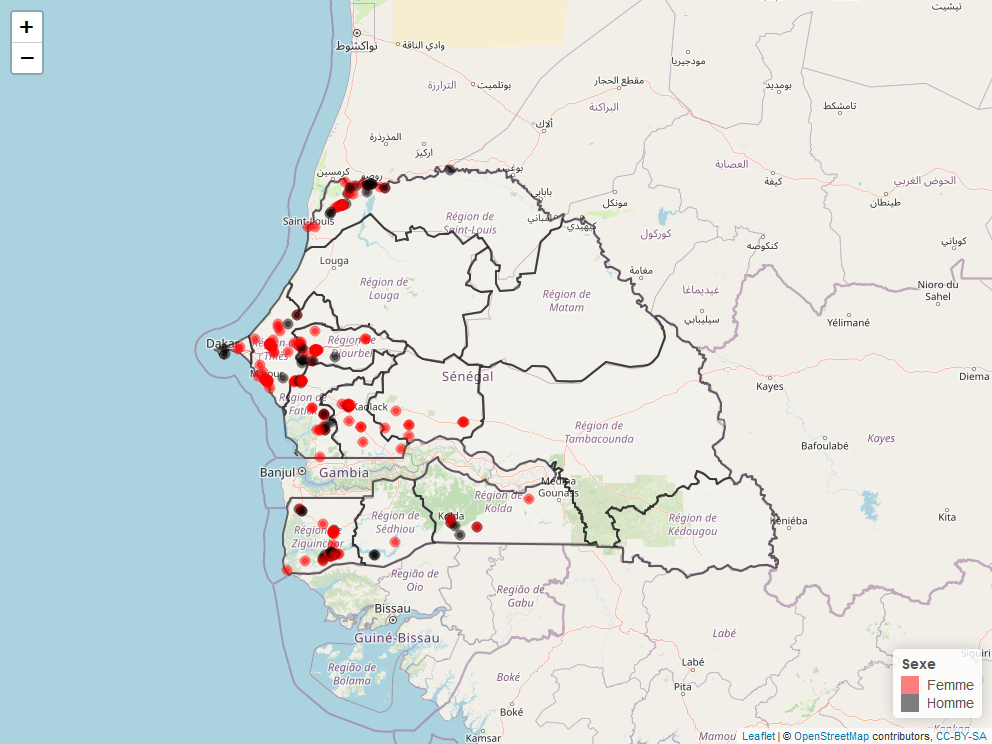
\includegraphics{TP-R-ESSAI_files/figure-latex/unnamed-chunk-9-1.png}

\hypertarget{ruxe9pruxe9sentation-spatial-des-pme-suivant-le-niveau-dinstruction}{%
\paragraph{1.3.3 réprésentation spatial des PME suivant le niveau
d'instruction}\label{ruxe9pruxe9sentation-spatial-des-pme-suivant-le-niveau-dinstruction}}

Ici, nous procédons de la meme façon qu'a la question 1.3.2

\begin{Shaded}
\begin{Highlighting}[]
\NormalTok{sen\_polyg }\OtherTok{=} \FunctionTok{getData}\NormalTok{(}\StringTok{"GADM"}\NormalTok{, }\AttributeTok{country=} \StringTok{"senegal"}\NormalTok{, }\AttributeTok{level =} \DecValTok{1}\NormalTok{)}
\end{Highlighting}
\end{Shaded}

\begin{verbatim}
## Warning in getData("GADM", country = "senegal", level = 1): getData will be removed in a future version of raster
## . Please use the geodata package instead
\end{verbatim}

\begin{Shaded}
\begin{Highlighting}[]
\CommentTok{\#Definition d\textquotesingle{}un jeu de 4 couleurs qui représentera chaque niveau scolaire.}
\NormalTok{color}\OtherTok{\textless{}{-}}\FunctionTok{colorFactor}\NormalTok{(}\FunctionTok{c}\NormalTok{(}\StringTok{"red"}\NormalTok{,}\StringTok{"black"}\NormalTok{,}\StringTok{"yellow"}\NormalTok{,}\StringTok{"green"}\NormalTok{),}\AttributeTok{domain=}\NormalTok{projet\_map}\SpecialCharTok{$}\NormalTok{q25) }
\CommentTok{\#Création d\textquotesingle{}une carte interactive}
\NormalTok{m1}\OtherTok{\textless{}{-}}\FunctionTok{leaflet}\NormalTok{(sen\_polyg) }\SpecialCharTok{\%\textgreater{}\%} \FunctionTok{addPolygons}\NormalTok{(}\AttributeTok{data =}\NormalTok{ sen\_polyg,}
                                     \AttributeTok{color =} \StringTok{"black"}\NormalTok{,}\AttributeTok{weight =} \DecValTok{4}\NormalTok{,}
  \AttributeTok{opacity =} \FloatTok{0.5}\NormalTok{,}
  \AttributeTok{fillColor =} \StringTok{"white"}\NormalTok{,}
  \AttributeTok{fillOpacity =} \FloatTok{0.1}\NormalTok{) }\SpecialCharTok{\%\textgreater{}\%}
  \FunctionTok{addCircleMarkers}\NormalTok{(}\AttributeTok{data=}\NormalTok{projet\_map,}\AttributeTok{color=}\SpecialCharTok{\textasciitilde{}}\FunctionTok{color}\NormalTok{(q25),}
    \AttributeTok{radius =} \DecValTok{3}\NormalTok{,}
     \CommentTok{\# Utilisation de couleurs différentes selon le sexe}
    \AttributeTok{fillOpacity =} \FloatTok{0.5}\NormalTok{,}
\NormalTok{  ) }\SpecialCharTok{\%\textgreater{}\%} 
  \FunctionTok{addTiles}\NormalTok{() }\SpecialCharTok{\%\textgreater{}\%} 
  \FunctionTok{addLegend}\NormalTok{(}\AttributeTok{position=}\StringTok{"bottomright"}\NormalTok{,}
            \AttributeTok{pal=}\NormalTok{color,}
            \AttributeTok{title=}\StringTok{"niveau d\textquotesingle{}instruction"}\NormalTok{,}\AttributeTok{values=}\NormalTok{projet\_map}\SpecialCharTok{$}\NormalTok{q25)}\CommentTok{\# positionnement de la légende à droite}


\CommentTok{\# Etant donné que le graphes est interactif il faut faire la capture d\textquotesingle{}écran}
\FunctionTok{saveWidget}\NormalTok{(m1,}\AttributeTok{file=}\StringTok{"q25.html"}\NormalTok{)}
\FunctionTok{webshot}\NormalTok{(}\StringTok{"q25.html"}\NormalTok{,}\StringTok{"q25.png"}\NormalTok{)}
\end{Highlighting}
\end{Shaded}

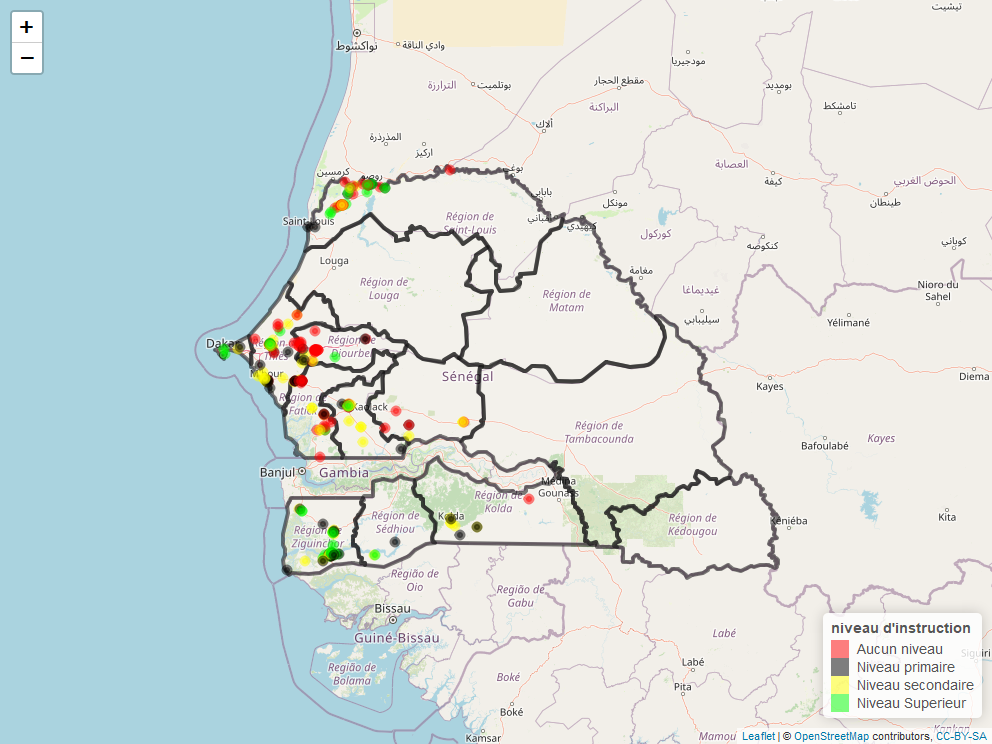
\includegraphics{TP-R-ESSAI_files/figure-latex/unnamed-chunk-10-1.png}

\hypertarget{faisons-une-analyse-spatiale-de-notre-choix}{%
\paragraph{1.3.4 faisons une analyse spatiale de notre
choix}\label{faisons-une-analyse-spatiale-de-notre-choix}}

repartition des PME suivant qu'ils soient propriétaires ou localtaires

\begin{Shaded}
\begin{Highlighting}[]
\NormalTok{sen\_polyg }\OtherTok{=} \FunctionTok{getData}\NormalTok{(}\StringTok{"GADM"}\NormalTok{, }\AttributeTok{country=} \StringTok{"senegal"}\NormalTok{, }\AttributeTok{level =} \DecValTok{1}\NormalTok{)}
\end{Highlighting}
\end{Shaded}

\begin{verbatim}
## Warning in getData("GADM", country = "senegal", level = 1): getData will be removed in a future version of raster
## . Please use the geodata package instead
\end{verbatim}

\begin{Shaded}
\begin{Highlighting}[]
\CommentTok{\# couleur réprésentative du genre de chaque chef des PME sur la carte}
\NormalTok{color\_Pro}\OtherTok{\textless{}{-}}\FunctionTok{colorFactor}\NormalTok{(}\FunctionTok{c}\NormalTok{(}\StringTok{"green"}\NormalTok{,}\StringTok{"red"}\NormalTok{),}\AttributeTok{domain=}\NormalTok{projet\_map}\SpecialCharTok{$}\NormalTok{q81)}
\CommentTok{\#création d\textquotesingle{}une carte interactive}
\NormalTok{m2}\OtherTok{\textless{}{-}}\FunctionTok{leaflet}\NormalTok{(sen\_polyg) }\SpecialCharTok{\%\textgreater{}\%} \FunctionTok{addPolygons}\NormalTok{(}\AttributeTok{data =}\NormalTok{ sen\_polyg,}
                                     \AttributeTok{color =} \StringTok{"black"}\NormalTok{,}\AttributeTok{weight =} \DecValTok{2}\NormalTok{, }\CommentTok{\#ajouter un polygone sur la carte}
  \AttributeTok{opacity =} \FloatTok{0.5}\NormalTok{,}
  \AttributeTok{fillColor =} \StringTok{"white"}\NormalTok{,}
  \AttributeTok{fillOpacity =} \FloatTok{0.1}\NormalTok{) }\SpecialCharTok{\%\textgreater{}\%}
  \FunctionTok{addCircleMarkers}\NormalTok{(}
    \AttributeTok{data=}\NormalTok{projet\_map,}
    \AttributeTok{radius =} \DecValTok{3}\NormalTok{,}
    \AttributeTok{color =} \FunctionTok{ifelse}\NormalTok{(projet\_map}\SpecialCharTok{$}\NormalTok{q81 }\SpecialCharTok{==} \StringTok{"Propriétaire"}\NormalTok{, }\StringTok{"green"}\NormalTok{, }\StringTok{"red"}\NormalTok{), }\CommentTok{\# Utilisation de couleurs différentes selon le sexe}
    \AttributeTok{fillOpacity =} \FloatTok{0.5}\NormalTok{,}
    \AttributeTok{popup =} \FunctionTok{ifelse}\NormalTok{(projet\_map}\SpecialCharTok{$}\NormalTok{q81 }\SpecialCharTok{==} \StringTok{"Propriétaire"}\NormalTok{, }\StringTok{"Propriétaire"}\NormalTok{, }\StringTok{"Locataire"}\NormalTok{) }
\NormalTok{  ) }\SpecialCharTok{\%\textgreater{}\%} 
  \FunctionTok{addTiles}\NormalTok{() }\SpecialCharTok{\%\textgreater{}\%} 
  \FunctionTok{addLegend}\NormalTok{(}\AttributeTok{position=}\StringTok{"bottomright"}\NormalTok{,}
            \AttributeTok{pal=}\NormalTok{color\_Pro,}
            \AttributeTok{title=}\StringTok{"propriétaire"}\NormalTok{,}\AttributeTok{values=}\NormalTok{projet\_map}\SpecialCharTok{$}\NormalTok{q81) }\CommentTok{\# ajouter une légende sur la carte}


\CommentTok{\# Etant donné que le graphes est interactif il faut faire la capture d\textquotesingle{}écran}
\FunctionTok{saveWidget}\NormalTok{(m2,}\AttributeTok{file=}\StringTok{"q81.html"}\NormalTok{)}
\FunctionTok{webshot}\NormalTok{(}\StringTok{"q81.html"}\NormalTok{,}\StringTok{"q81.png"}\NormalTok{)}
\end{Highlighting}
\end{Shaded}

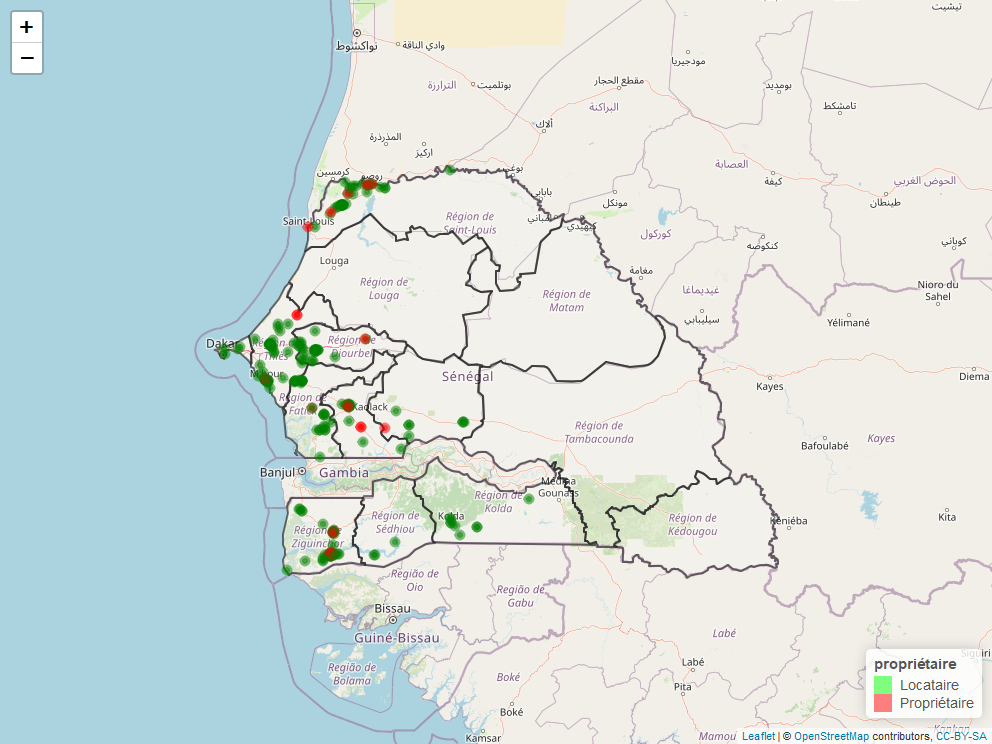
\includegraphics{TP-R-ESSAI_files/figure-latex/unnamed-chunk-11-1.png}

\hypertarget{partie-2-nettoyage-et-gestion-des-donnees-importation-de-la-base-de}{%
\section{PARTIE 2: NETTOYAGE ET GESTION DES DONNEES importation de la
base
de}\label{partie-2-nettoyage-et-gestion-des-donnees-importation-de-la-base-de}}

Ici nous ferons usage de la Base\_Partie 2 sur laquelle nous renommerons
ou créerons des variables, créerons un nuage de points et éffectuerons
un ensemble de testes.

\hypertarget{importation-de-base_partie-2}{%
\subsection{Importation de Base\_partie
2}\label{importation-de-base_partie-2}}

pour effectuer n'importe quelle opération sur la base il est nécéssaire
de l'importée.

\begin{Shaded}
\begin{Highlighting}[]
\NormalTok{projetN}\OtherTok{\textless{}{-}} \FunctionTok{read\_excel}\NormalTok{(}\StringTok{"Base\_Partie 2.xlsx"}\NormalTok{,}
                    \AttributeTok{range=}\ConstantTok{NULL}\NormalTok{,}
                    \AttributeTok{col\_names =} \ConstantTok{TRUE}\NormalTok{,}
                    \AttributeTok{col\_types =} \ConstantTok{NULL}\NormalTok{,}
\NormalTok{                    )}
\end{Highlighting}
\end{Shaded}

\hypertarget{nettoyage-et-gestion-des-donnuxe9es}{%
\subsubsection{2.1 Nettoyage et gestion des
données}\label{nettoyage-et-gestion-des-donnuxe9es}}

Ici, nous effectuerons certaines tache sur les variables et manipulerons
les données manquantes

\hypertarget{renommons-la-variable-country_destination-en-destination-et-duxe9finissons-les-valeurs-nuxe9gatives-comme-manquantes.}{%
\paragraph{2.1.1 Renommons la variable ``country\_destination'' en
``destination'' et définissons les valeurs négatives comme
manquantes.}\label{renommons-la-variable-country_destination-en-destination-et-duxe9finissons-les-valeurs-nuxe9gatives-comme-manquantes.}}

Pour éxécuter cette tache, nous fairerons usage de la fonction
\textbf{rename} de \textbf{dplyr}.

\begin{Shaded}
\begin{Highlighting}[]
\NormalTok{projetN}\OtherTok{\textless{}{-}}\NormalTok{ projetN }\SpecialCharTok{\%\textgreater{}\%}\NormalTok{ dplyr}\SpecialCharTok{::}\FunctionTok{rename}\NormalTok{(}\AttributeTok{destination=}\NormalTok{ country\_destination)}
\CommentTok{\#filtrage de toutes les valeurs négatives du data frame projet et leur remplacement par les NA supprimant ainsi les valeurs négatives de la base.}
\NormalTok{projetN[projetN }\SpecialCharTok{\textless{}} \DecValTok{0}\NormalTok{] }\OtherTok{\textless{}{-}} \ConstantTok{NA} 
\end{Highlighting}
\end{Shaded}

\hypertarget{cruxe9ons-une-nouvelle-variable-contenant-des-tranches-duxe2ge-de-5-ans-en-utilisant-la-variable-age.}{%
\paragraph{2.1.2 Créons une nouvelle variable contenant des tranches
d'âge de 5 ans en utilisant la variable
``age''.}\label{cruxe9ons-une-nouvelle-variable-contenant-des-tranches-duxe2ge-de-5-ans-en-utilisant-la-variable-age.}}

la variriable age possédant des données abhérantes, nous allons d'abord
chercher à éliminer l'effet de ces valeurs. pour cela, nous procéderons
à une imputation par la médiane. Le choix de cette méthode se justifie
par le faite que la médiane est moins sensible au valeurs abhérantes.

\begin{Shaded}
\begin{Highlighting}[]
\CommentTok{\# calcul du premier et du troisième quartille qui serviront à déterminer l\textquotesingle{}écart interquartile}
\NormalTok{q1 }\OtherTok{\textless{}{-}} \FunctionTok{quantile}\NormalTok{(projetN}\SpecialCharTok{$}\NormalTok{age, }\FloatTok{0.25}\NormalTok{)}
\NormalTok{q3 }\OtherTok{\textless{}{-}} \FunctionTok{quantile}\NormalTok{(projetN}\SpecialCharTok{$}\NormalTok{age, }\FloatTok{0.75}\NormalTok{)}
\CommentTok{\#calcul de l\textquotesingle{}écart interquartile iqr.}
\NormalTok{iqr }\OtherTok{\textless{}{-}}\NormalTok{ q3 }\SpecialCharTok{{-}}\NormalTok{ q1      }
\CommentTok{\# calcul des bornes inférieurs et supérieurs qui nous servirrons à détecter les  valeurs aberrante}
\NormalTok{min1 }\OtherTok{\textless{}{-}}\NormalTok{ q1 }\SpecialCharTok{{-}} \FloatTok{1.5} \SpecialCharTok{*}\NormalTok{ iqr}
\NormalTok{max1 }\OtherTok{\textless{}{-}}\NormalTok{ q3 }\SpecialCharTok{+} \FloatTok{1.5} \SpecialCharTok{*}\NormalTok{ iqr}

\CommentTok{\#  créons une nouvelle colone val\_aber pour stocker les valeurs aberrantes remplacées par la médiane}
\NormalTok{projetN}\SpecialCharTok{$}\NormalTok{val\_aber }\OtherTok{\textless{}{-}} \FunctionTok{ifelse}\NormalTok{((projetN}\SpecialCharTok{$}\NormalTok{age }\SpecialCharTok{\textless{}}\NormalTok{ min1) }\SpecialCharTok{|}\NormalTok{ (projetN}\SpecialCharTok{$}\NormalTok{age }\SpecialCharTok{\textgreater{}}\NormalTok{ max1),}
                                    \FunctionTok{median}\NormalTok{(projetN}\SpecialCharTok{$}\NormalTok{age,}\AttributeTok{na.rm =}\ConstantTok{TRUE}\NormalTok{ ),}
\NormalTok{                                    projetN}\SpecialCharTok{$}\NormalTok{age)}
\CommentTok{\#créons les bornes pour les tranches d\textquotesingle{}age}
\NormalTok{bornes}\OtherTok{\textless{}{-}}\FunctionTok{seq}\NormalTok{( }\FunctionTok{min}\NormalTok{(projetN}\SpecialCharTok{$}\NormalTok{val\_aber),}\FunctionTok{max}\NormalTok{(projetN}\SpecialCharTok{$}\NormalTok{val\_aber),}\AttributeTok{by=}\DecValTok{5}\NormalTok{)}
\CommentTok{\# création de la variable "tranche\_age" contenant les tranches d\textquotesingle{}age}
\NormalTok{projetN }\OtherTok{\textless{}{-}} \FunctionTok{within}\NormalTok{(projetN, tranche\_age }\OtherTok{\textless{}{-}} \FunctionTok{cut}\NormalTok{(val\_aber, }\AttributeTok{breaks =}\NormalTok{ bornes))}
\CommentTok{\#afficher la table des tranches d\textquotesingle{}ages}
\FunctionTok{table}\NormalTok{(projetN}\SpecialCharTok{$}\NormalTok{tranche\_age)}
\end{Highlighting}
\end{Shaded}

\begin{verbatim}
## 
## (15,20] (20,25] (25,30] (30,35] (35,40] 
##      20      37      22      10       7
\end{verbatim}

\hypertarget{cruxe9er-une-nouvelle-variable-contenant-le-nombre-dentretiens-ruxe9alisuxe9s-par-chaque-agent-recenseur.}{%
\paragraph{2.1.3 Créer une nouvelle variable contenant le nombre
d'entretiens réalisés par chaque agent
recenseur.}\label{cruxe9er-une-nouvelle-variable-contenant-le-nombre-dentretiens-ruxe9alisuxe9s-par-chaque-agent-recenseur.}}

Pour cela, nous créerons la table nbre\_entre\_ag contiendra le nombre
d'occurrences de chaque valeur unique dans la colonne enumerator.la
fonction match ici, recherche les positions des valeurs de
projetN\$enumerator dans names(nbre\_entre\_ag) (les noms des valeurs
uniques dans la table nbre\_entre\_ag). Elle retourne un vecteur avec
les positions correspondantes. pour chaque valeur de
enuméretor,nbre\_entre\_ag{[}match(\ldots){]} renvoie le nombre
d'entretients correspondant à cette valeur.

\begin{Shaded}
\begin{Highlighting}[]
\NormalTok{nbre\_entre\_ag }\OtherTok{\textless{}{-}} \FunctionTok{table}\NormalTok{(projetN}\SpecialCharTok{$}\NormalTok{enumerator)}
\CommentTok{\#création d\textquotesingle{}une nouvelle colone dans le projetN.}
\NormalTok{projetN}\SpecialCharTok{$}\NormalTok{nbre\_entretien}\OtherTok{\textless{}{-}}\NormalTok{nbre\_entre\_ag[}\FunctionTok{match}\NormalTok{(projetN}\SpecialCharTok{$}\NormalTok{enumerator,                                               }\FunctionTok{names}\NormalTok{(nbre\_entre\_ag))]}
\end{Highlighting}
\end{Shaded}

\hypertarget{cruxe9er-une-nouvelle-variable-qui-affecte-aluxe9atoirement-chaque-ruxe9pondant-uxe0-un-groupe-de-traitement-1-ou-de-controle-0.}{%
\paragraph{2.1.4 Créer une nouvelle variable qui affecte aléatoirement
chaque répondant à un groupe de traitement (1) ou de controle
(0).}\label{cruxe9er-une-nouvelle-variable-qui-affecte-aluxe9atoirement-chaque-ruxe9pondant-uxe0-un-groupe-de-traitement-1-ou-de-controle-0.}}

Pour cela nous allons d'abord déterminer le nombre de ligne de projetN
avec la fonction \textbf{nrow}. ensuite, nous ferons usage de la
fonction sample qui génèrera aléatoirement soit 0, soit 1 à chaque
différentes ligne.

\begin{Shaded}
\begin{Highlighting}[]
\CommentTok{\#Détermination du nombre de ligne du data frame projetN}
\NormalTok{nombre\_total\_respondants }\OtherTok{\textless{}{-}} \FunctionTok{nrow}\NormalTok{(projetN)}
\CommentTok{\#Génèration aléatoire des valeur 0 et 1 aux différentes lignes.}
\NormalTok{projetN}\SpecialCharTok{$}\NormalTok{alea\_affect }\OtherTok{\textless{}{-}} \FunctionTok{sample}\NormalTok{(}\FunctionTok{c}\NormalTok{(}\DecValTok{1}\NormalTok{, }\DecValTok{0}\NormalTok{), }\AttributeTok{size =}\NormalTok{ nombre\_total\_respondants, }\AttributeTok{replace =} \ConstantTok{TRUE}\NormalTok{,}\AttributeTok{prob=}\ConstantTok{NULL}\NormalTok{)}
\end{Highlighting}
\end{Shaded}

\hypertarget{fusionner-la-taille-de-la-population-de-chaque-district-feuille-2-avec-lensemble-de-donnuxe9es-feuille-1-afin-que-toutes-les-personnes-interroguxe9es-aient-une-valeur-correspondante-repruxe9sentant-la-taille-de-la-population-du-district-dans-lequel-elles-vivent.}{%
\paragraph{2.1.5 Fusionner la taille de la population de chaque district
(feuille 2) avec l'ensemble de données (feuille 1) afin que toutes les
personnes interrogées aient une valeur correspondante représentant la
taille de la population du district dans lequel elles
vivent.}\label{fusionner-la-taille-de-la-population-de-chaque-district-feuille-2-avec-lensemble-de-donnuxe9es-feuille-1-afin-que-toutes-les-personnes-interroguxe9es-aient-une-valeur-correspondante-repruxe9sentant-la-taille-de-la-population-du-district-dans-lequel-elles-vivent.}}

La feuille une de Base\_partie 2 étant déja importée, nous importerons
maintenant uniquement la feuille deux de ce fichier.Puis à l'aide de la
fonction merge nous aurons le résultat souhaiter.

\begin{Shaded}
\begin{Highlighting}[]
\CommentTok{\#importation de la feuille 2 de Base\_partie 2}
\NormalTok{projetN2}\OtherTok{\textless{}{-}} \FunctionTok{read\_excel}\NormalTok{(}\StringTok{"Base\_Partie 2.xlsx"}\NormalTok{,}\AttributeTok{sheet=}\StringTok{"district"}\NormalTok{)}
\CommentTok{\#Création du data frame fusion qui contient la fusion des deux feuilles.}
\NormalTok{fusion }\OtherTok{\textless{}{-}} \FunctionTok{merge}\NormalTok{(projetN, projetN2, }\AttributeTok{by =} \StringTok{"district"}\NormalTok{, }\AttributeTok{all.x =} \ConstantTok{TRUE}\NormalTok{)}
\end{Highlighting}
\end{Shaded}

\hypertarget{calculer-la-duruxe9e-de-lentretien-et-indiquer-la-duruxe9e-moyenne-de-lentretien-par-enquuxeateur.}{%
\paragraph{2.1.6 Calculer la durée de l'entretien et indiquer la durée
moyenne de l'entretien par
enquêteur.}\label{calculer-la-duruxe9e-de-lentretien-et-indiquer-la-duruxe9e-moyenne-de-lentretien-par-enquuxeateur.}}

Pour cela nous créerons d'abord une varible qui contient la durée de
chaque entretient.Ensuite à l'aide ces durées, nous déterminerons la
durée moyenne par enqueteur.

\begin{Shaded}
\begin{Highlighting}[]
\NormalTok{projetN}\SpecialCharTok{$}\NormalTok{starttime }\OtherTok{\textless{}{-}} \FunctionTok{as.POSIXct}\NormalTok{(projetN}\SpecialCharTok{$}\NormalTok{starttime , }\AttributeTok{format =} \StringTok{"\%Y{-}\%m{-}\%d \%H:\%M"}\NormalTok{)}
\NormalTok{projetN}\SpecialCharTok{$}\NormalTok{endtime }\OtherTok{\textless{}{-}} \FunctionTok{as.POSIXct}\NormalTok{(projetN}\SpecialCharTok{$}\NormalTok{endtime, }\AttributeTok{format =} \StringTok{"\%Y{-}\%m{-}\%d \%H:\%M"}\NormalTok{)}

\CommentTok{\# Calculer la durée de l\textquotesingle{}entretien (en minutes)}
\NormalTok{projetN}\SpecialCharTok{$}\NormalTok{duree\_entretien }\OtherTok{\textless{}{-}} \FunctionTok{difftime}\NormalTok{(projetN}\SpecialCharTok{$}\NormalTok{endtime, projetN}\SpecialCharTok{$}\NormalTok{starttime, }\AttributeTok{units =} \StringTok{"mins"}\NormalTok{)}

\CommentTok{\# Calculer la durée moyenne de l\textquotesingle{}entretien par enquêteur}
\NormalTok{dur\_moy\_enq }\OtherTok{\textless{}{-}} \FunctionTok{aggregate}\NormalTok{(projetN}\SpecialCharTok{$}\NormalTok{duree\_entretien,}
                                         \AttributeTok{by =} \FunctionTok{list}\NormalTok{(}\AttributeTok{enqueteur =}\NormalTok{ projetN}\SpecialCharTok{$}\NormalTok{enumerator),}
                                         \AttributeTok{FUN =}\NormalTok{ mean)}

\CommentTok{\# Renommer les colonnes du résultat}
\FunctionTok{colnames}\NormalTok{(dur\_moy\_enq) }\OtherTok{\textless{}{-}} \FunctionTok{c}\NormalTok{(}\StringTok{"enqueteur"}\NormalTok{, }\StringTok{"duree\_moyenne\_entretien"}\NormalTok{)}

\CommentTok{\# Afficher le résultat}
\FunctionTok{print}\NormalTok{(dur\_moy\_enq)}
\end{Highlighting}
\end{Shaded}

\begin{verbatim}
##    enqueteur duree_moyenne_entretien
## 1          1           68.14667 mins
## 2          4           36.48333 mins
## 3          5           33.55833 mins
## 4          6           25.84667 mins
## 5          7           37.16429 mins
## 6          8           40.13056 mins
## 7          9          114.76667 mins
## 8         10           55.27667 mins
## 9         11           33.48333 mins
## 10        12           48.16667 mins
## 11        13           31.59583 mins
## 12        14           25.56111 mins
## 13        15           28.65000 mins
## 14        17           29.28611 mins
## 15        18           36.85833 mins
## 16        20           28.76852 mins
\end{verbatim}

\hypertarget{renommez-toutes-les-variables-de-lensemble-de-donnuxe9es-en-ajoutant-le-pruxe9fixe-endline_}{%
\paragraph{2.1.7 Renommez toutes les variables de l'ensemble de données
en ajoutant le préfixe
``endline\_''}\label{renommez-toutes-les-variables-de-lensemble-de-donnuxe9es-en-ajoutant-le-pruxe9fixe-endline_}}

Ici, nous ferons usage de la fonction paste() qui est utilisée pour
créer un nouveau vecteur de noms de colonnes en ajoutant le préfixe
``endline\_'' à chaque nom de colonne existant. Le paramètre sep =
``\,'' spécifie que les éléments sont concaténés sans espace entre le
préfixe et les noms de colonnes existants.

\begin{Shaded}
\begin{Highlighting}[]
\CommentTok{\# Renommer les variables en ajoutant le préfixe "endline\_"}
\NormalTok{new\_names }\OtherTok{\textless{}{-}} \FunctionTok{paste}\NormalTok{(}\StringTok{"endline\_"}\NormalTok{, }\FunctionTok{names}\NormalTok{(projetN), }\AttributeTok{sep =} \StringTok{""}\NormalTok{)}
\CommentTok{\#attribution au nouvel objet de noms de colonnes, new\_names, à l\textquotesingle{}objet de données projetN.}
\FunctionTok{names}\NormalTok{(projetN) }\OtherTok{\textless{}{-}}\NormalTok{ new\_names}
\end{Highlighting}
\end{Shaded}

\hypertarget{analyse-et-visualisation-des-donnees}{%
\subsubsection{2.2 ANALYSE ET VISUALISATION DES
DONNEES}\label{analyse-et-visualisation-des-donnees}}

Dans cette section nous ferons ressortir quelques tableaux,et nous
éffectuerons également quelques tests.

\hypertarget{cruxe9ez-un-tableau-ruxe9capitulatif-contenant-luxe2ge-moyen-et-le-nombre-moyen-denfants-par-district.}{%
\paragraph{2.2.1 Créez un tableau récapitulatif contenant l'âge moyen et
le nombre moyen d'enfants par
district.}\label{cruxe9ez-un-tableau-ruxe9capitulatif-contenant-luxe2ge-moyen-et-le-nombre-moyen-denfants-par-district.}}

Comme resultat nous un tableau ayant en colonne les différents discrits
et en ligne les variables endline\_val\_aber, endline\_children\_num .
les valeurs du tableau contiendrons donc l'age moyen et le nombre moyen
d'enfants par discrit. NB: Nous avons travailler avec la variable
endline\_val\_aber au lieu de endline\_age parceque sur
endline\_val\_aber nous avons déjà gérer le problème des valeurs
abérantes.

\begin{Shaded}
\begin{Highlighting}[]
\NormalTok{projetN }\SpecialCharTok{\%\textgreater{}\%}
  \CommentTok{\#création du tableau à l\textquotesingle{}aide de la fonction tbl\_summary de gtsummary}
\NormalTok{  gtsummary}\SpecialCharTok{::}\FunctionTok{tbl\_summary}\NormalTok{(}
    \AttributeTok{include =} \FunctionTok{c}\NormalTok{(endline\_val\_aber,endline\_children\_num ),}
    \AttributeTok{by =}\NormalTok{endline\_district,}
    \AttributeTok{statistic =} \FunctionTok{all\_continuous}\NormalTok{() }\SpecialCharTok{\textasciitilde{}} \StringTok{" \{mean\} "}
\NormalTok{  )}\SpecialCharTok{\%\textgreater{}\%}
  \FunctionTok{modify\_header}\NormalTok{(label }\SpecialCharTok{\textasciitilde{}} \StringTok{"**Variables**"}\NormalTok{) }\SpecialCharTok{\%\textgreater{}\%}
  \FunctionTok{modify\_spanning\_header}\NormalTok{(}\FunctionTok{c}\NormalTok{(}\StringTok{"stat\_1"}\NormalTok{, }\StringTok{"stat\_2"}\NormalTok{) }\SpecialCharTok{\textasciitilde{}} \StringTok{"**district**"}\NormalTok{) }\SpecialCharTok{\%\textgreater{}\%}
  \CommentTok{\#afficher le titre du tableau}
  \FunctionTok{modify\_caption}\NormalTok{(}\StringTok{"**Tableau recap age et nombre moyen d\textquotesingle{}\textquotesingle{}enfant par discrit**"}\NormalTok{) }\SpecialCharTok{\%\textgreater{}\%}
  \CommentTok{\# Mettre les variables en gras}
  \FunctionTok{bold\_labels}\NormalTok{()}
\end{Highlighting}
\end{Shaded}

\begin{verbatim}
## Table printed with `knitr::kable()`, not {gt}. Learn why at
## https://www.danieldsjoberg.com/gtsummary/articles/rmarkdown.html
## To suppress this message, include `message = FALSE` in code chunk header.
\end{verbatim}

\begin{longtable}[]{@{}
  >{\raggedright\arraybackslash}p{(\columnwidth - 16\tabcolsep) * \real{0.1786}}
  >{\centering\arraybackslash}p{(\columnwidth - 16\tabcolsep) * \real{0.1000}}
  >{\centering\arraybackslash}p{(\columnwidth - 16\tabcolsep) * \real{0.1071}}
  >{\centering\arraybackslash}p{(\columnwidth - 16\tabcolsep) * \real{0.1000}}
  >{\centering\arraybackslash}p{(\columnwidth - 16\tabcolsep) * \real{0.1000}}
  >{\centering\arraybackslash}p{(\columnwidth - 16\tabcolsep) * \real{0.1000}}
  >{\centering\arraybackslash}p{(\columnwidth - 16\tabcolsep) * \real{0.1071}}
  >{\centering\arraybackslash}p{(\columnwidth - 16\tabcolsep) * \real{0.1000}}
  >{\centering\arraybackslash}p{(\columnwidth - 16\tabcolsep) * \real{0.1071}}@{}}
\caption{\textbf{Tableau recap age et nombre moyen d'\,'enfant par
discrit}}\tabularnewline
\toprule\noalign{}
\begin{minipage}[b]{\linewidth}\raggedright
\textbf{Variables}
\end{minipage} & \begin{minipage}[b]{\linewidth}\centering
\textbf{1}, N = 8
\end{minipage} & \begin{minipage}[b]{\linewidth}\centering
\textbf{2}, N = 27
\end{minipage} & \begin{minipage}[b]{\linewidth}\centering
\textbf{3}, N = 8
\end{minipage} & \begin{minipage}[b]{\linewidth}\centering
\textbf{4}, N = 5
\end{minipage} & \begin{minipage}[b]{\linewidth}\centering
\textbf{5}, N = 6
\end{minipage} & \begin{minipage}[b]{\linewidth}\centering
\textbf{6}, N = 26
\end{minipage} & \begin{minipage}[b]{\linewidth}\centering
\textbf{7}, N = 6
\end{minipage} & \begin{minipage}[b]{\linewidth}\centering
\textbf{8}, N = 11
\end{minipage} \\
\midrule\noalign{}
\endfirsthead
\toprule\noalign{}
\begin{minipage}[b]{\linewidth}\raggedright
\textbf{Variables}
\end{minipage} & \begin{minipage}[b]{\linewidth}\centering
\textbf{1}, N = 8
\end{minipage} & \begin{minipage}[b]{\linewidth}\centering
\textbf{2}, N = 27
\end{minipage} & \begin{minipage}[b]{\linewidth}\centering
\textbf{3}, N = 8
\end{minipage} & \begin{minipage}[b]{\linewidth}\centering
\textbf{4}, N = 5
\end{minipage} & \begin{minipage}[b]{\linewidth}\centering
\textbf{5}, N = 6
\end{minipage} & \begin{minipage}[b]{\linewidth}\centering
\textbf{6}, N = 26
\end{minipage} & \begin{minipage}[b]{\linewidth}\centering
\textbf{7}, N = 6
\end{minipage} & \begin{minipage}[b]{\linewidth}\centering
\textbf{8}, N = 11
\end{minipage} \\
\midrule\noalign{}
\endhead
\bottomrule\noalign{}
\endlastfoot
\textbf{endline\_val\_aber} & 27.3 & 26.5 & 26.1 & 26.0 & 24.3 & 23.2 &
25.0 & 24.6 \\
\textbf{endline\_children\_num} & & & & & & & & \\
0 & 4 (50\%) & 17 (63\%) & 8 (100\%) & 5 (100\%) & 4 (67\%) & 23 (88\%)
& 5 (83\%) & 7 (64\%) \\
1 & 1 (13\%) & 3 (11\%) & 0 (0\%) & 0 (0\%) & 1 (17\%) & 3 (12\%) & 1
(17\%) & 0 (0\%) \\
2 & 1 (13\%) & 3 (11\%) & 0 (0\%) & 0 (0\%) & 1 (17\%) & 0 (0\%) & 0
(0\%) & 1 (9.1\%) \\
3 & 0 (0\%) & 3 (11\%) & 0 (0\%) & 0 (0\%) & 0 (0\%) & 0 (0\%) & 0 (0\%)
& 2 (18\%) \\
4 & 1 (13\%) & 0 (0\%) & 0 (0\%) & 0 (0\%) & 0 (0\%) & 0 (0\%) & 0 (0\%)
& 0 (0\%) \\
5 & 1 (13\%) & 1 (3.7\%) & 0 (0\%) & 0 (0\%) & 0 (0\%) & 0 (0\%) & 0
(0\%) & 0 (0\%) \\
6 & 0 (0\%) & 0 (0\%) & 0 (0\%) & 0 (0\%) & 0 (0\%) & 0 (0\%) & 0 (0\%)
& 1 (9.1\%) \\
\end{longtable}

\hypertarget{testons-si-la-diffuxe9rence-duxe2ge-entre-les-sexes-est-statistiquement-significative-au-niveau-de-5-.}{%
\paragraph{2.2.2 Testons si la différence d'âge entre les sexes est
statistiquement significative au niveau de 5
\%.}\label{testons-si-la-diffuxe9rence-duxe2ge-entre-les-sexes-est-statistiquement-significative-au-niveau-de-5-.}}

D'après le test, on obtient une pie-value de \textbf{0.061} qui est
supérieur à 5\% donc la différence d'age entre les sexes n'est pas
statistiquement significatif.

\begin{Shaded}
\begin{Highlighting}[]
\NormalTok{projetN }\SpecialCharTok{\%\textgreater{}\%}
\NormalTok{  gtsummary}\SpecialCharTok{::}\FunctionTok{tbl\_summary}\NormalTok{(}
    \AttributeTok{include =}\NormalTok{ endline\_val\_aber,}
    \AttributeTok{by =}\NormalTok{ endline\_sex}
\NormalTok{  ) }\SpecialCharTok{\%\textgreater{}\%}
  \CommentTok{\#idiquons la différence entre les différentes catégories à l\textquotesingle{}aide de la fonction add\_difference()}
  \FunctionTok{add\_difference}\NormalTok{()}
\end{Highlighting}
\end{Shaded}

\begin{verbatim}
## Table printed with `knitr::kable()`, not {gt}. Learn why at
## https://www.danieldsjoberg.com/gtsummary/articles/rmarkdown.html
## To suppress this message, include `message = FALSE` in code chunk header.
\end{verbatim}

\begin{longtable}[]{@{}
  >{\raggedright\arraybackslash}p{(\columnwidth - 10\tabcolsep) * \real{0.1939}}
  >{\centering\arraybackslash}p{(\columnwidth - 10\tabcolsep) * \real{0.1939}}
  >{\centering\arraybackslash}p{(\columnwidth - 10\tabcolsep) * \real{0.1939}}
  >{\centering\arraybackslash}p{(\columnwidth - 10\tabcolsep) * \real{0.1633}}
  >{\centering\arraybackslash}p{(\columnwidth - 10\tabcolsep) * \real{0.1224}}
  >{\centering\arraybackslash}p{(\columnwidth - 10\tabcolsep) * \real{0.1327}}@{}}
\toprule\noalign{}
\begin{minipage}[b]{\linewidth}\raggedright
\textbf{Characteristic}
\end{minipage} & \begin{minipage}[b]{\linewidth}\centering
\textbf{0}, N = 86
\end{minipage} & \begin{minipage}[b]{\linewidth}\centering
\textbf{1}, N = 11
\end{minipage} & \begin{minipage}[b]{\linewidth}\centering
\textbf{Difference}
\end{minipage} & \begin{minipage}[b]{\linewidth}\centering
\textbf{95\% CI}
\end{minipage} & \begin{minipage}[b]{\linewidth}\centering
\textbf{p-value}
\end{minipage} \\
\midrule\noalign{}
\endhead
\bottomrule\noalign{}
\endlastfoot
endline\_val\_aber & 24.0 (21.0, 29.0) & 21.0 (18.0, 23.0) & 3.4 &
-0.17, 6.9 & 0.061 \\
\end{longtable}

\hypertarget{cruxe9er-un-nuage-de-points-de-luxe2ge-en-fonction-du-nombre-denfants}{%
\paragraph{2.2.3 Créer un nuage de points de l'âge en fonction du nombre
d'enfants}\label{cruxe9er-un-nuage-de-points-de-luxe2ge-en-fonction-du-nombre-denfants}}

Pour cette question nous ferrons usage de ggplot pour avoir un nuage de
point un peu jolie.

\begin{Shaded}
\begin{Highlighting}[]
\FunctionTok{ggplot}\NormalTok{(projetN) }\SpecialCharTok{+}
  \FunctionTok{aes}\NormalTok{(}\AttributeTok{x =}\NormalTok{ endline\_val\_aber, }\AttributeTok{y =}\NormalTok{endline\_children\_num ) }\SpecialCharTok{+}
  \FunctionTok{geom\_point}\NormalTok{(}\AttributeTok{color =} \StringTok{"blue"}\NormalTok{, }\AttributeTok{alpha =} \FloatTok{0.7}\NormalTok{) }\SpecialCharTok{+}
  \FunctionTok{labs}\NormalTok{(}\AttributeTok{x =} \StringTok{"Âge"}\NormalTok{, }\AttributeTok{y =} \StringTok{"Nombre d\textquotesingle{}enfants"}\NormalTok{, }\AttributeTok{title =} \StringTok{"Nuage de points : Âge en fonction du nombre d\textquotesingle{}enfants"}\NormalTok{)}\CommentTok{\# Donne l\textquotesingle{}institulé des différents axes ainsi que le titre du graphique.}
\end{Highlighting}
\end{Shaded}

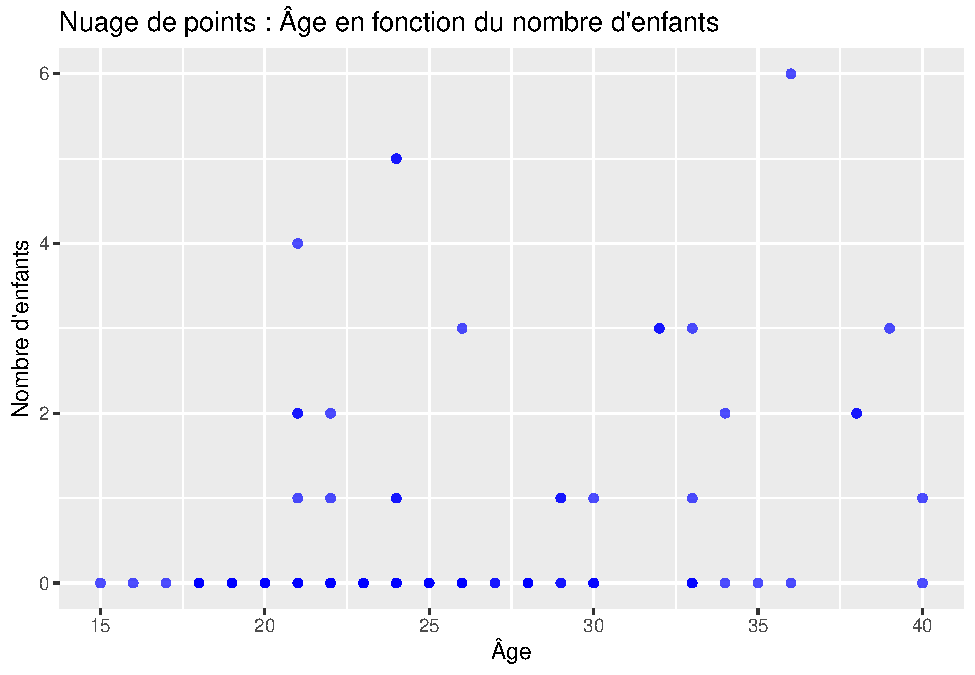
\includegraphics{TP-R-ESSAI_files/figure-latex/unnamed-chunk-22-1.pdf}

\hypertarget{la-variable-intention-indiquons-si-les-migrants-potentiels-ont-lintention-de-migrer-sur-une-uxe9chelle-de-1-uxe0-7.-estimons-leffet-de-lappartenance-au-groupe-de-traitement-sur-lintention-de-migrer.}{%
\paragraph{2.2.4 La variable ``intention'' indiquons si les migrants
potentiels ont l'intention de migrer sur une échelle de 1 à 7. Estimons
l'effet de l'appartenance au groupe de traitement sur l'intention de
migrer.}\label{la-variable-intention-indiquons-si-les-migrants-potentiels-ont-lintention-de-migrer-sur-une-uxe9chelle-de-1-uxe0-7.-estimons-leffet-de-lappartenance-au-groupe-de-traitement-sur-lintention-de-migrer.}}

Pour l'estimation, nous allons effectuer un test à l'aide d'un model de
regression linéaire simple.

\textbf{Interprétation du résultat}: le coefficient beta étant positif,
une augmentation de l'appartenance au groupe de traitement entraine une
augmentation de l'intention de migrer. La pie-Value étant supérieur à
\textbf{0.9}, elle est élevée ce qui fait comprendre que l'effet de
l'appartenance au groupe de migrants potentiel sur l'intension de migrer
n'est pas statistiquement significatif et que les différences entre les
groupes pourraient être attribuées au hasard. L'interval de confiance
étant de \textbf{0.7} nous indique que l'estimation est moins précise.

\begin{Shaded}
\begin{Highlighting}[]
\CommentTok{\#lm nécessaire pour éffectuer de la regression}
\NormalTok{model }\OtherTok{\textless{}{-}} \FunctionTok{lm}\NormalTok{(endline\_intention }\SpecialCharTok{\textasciitilde{}}\NormalTok{endline\_alea\_affect , }\AttributeTok{data =}\NormalTok{ projetN)}
\FunctionTok{tbl\_regression}\NormalTok{(model) }\CommentTok{\#permet d\textquotesingle{}afficher le tableaude regression}
\end{Highlighting}
\end{Shaded}

\begin{verbatim}
## Table printed with `knitr::kable()`, not {gt}. Learn why at
## https://www.danieldsjoberg.com/gtsummary/articles/rmarkdown.html
## To suppress this message, include `message = FALSE` in code chunk header.
\end{verbatim}

\begin{longtable}[]{@{}lccc@{}}
\toprule\noalign{}
\textbf{Characteristic} & \textbf{Beta} & \textbf{95\% CI} &
\textbf{p-value} \\
\midrule\noalign{}
\endhead
\bottomrule\noalign{}
\endlastfoot
endline\_alea\_affect & -0.11 & -0.81, 0.58 & 0.7 \\
\end{longtable}

\hypertarget{cruxe9ez-un-tableau-de-ruxe9gression-avec-3-moduxe8les.-les-ruxe9sultats-des-trois-moduxe8les-doivent-uxeatre-affichuxe9s-dans-un-seul-tableau.}{%
\paragraph{2.2.5 Créez un tableau de régression avec 3 modèles. Les
résultats des trois modèles doivent être affichés dans un seul
tableau.}\label{cruxe9ez-un-tableau-de-ruxe9gression-avec-3-moduxe8les.-les-ruxe9sultats-des-trois-moduxe8les-doivent-uxeatre-affichuxe9s-dans-un-seul-tableau.}}

Etant donné que nous n'avons pas encore les baggages nécessaires pour
les interprétations des modéles, dans cette partie nous nous limiterrons
à la présentation du resultat demandé.

\begin{Shaded}
\begin{Highlighting}[]
\CommentTok{\#MODEL A:Modèle vide {-} Effet du traitement sur les intentions}
\NormalTok{modele\_A}\OtherTok{\textless{}{-}}\FunctionTok{lm}\NormalTok{(endline\_intention }\SpecialCharTok{\textasciitilde{}}\NormalTok{endline\_alea\_affect , }\AttributeTok{data =}\NormalTok{ projetN)}
\NormalTok{mod1}\OtherTok{\textless{}{-}}\FunctionTok{tbl\_regression}\NormalTok{(modele\_A)}

\CommentTok{\#Model B: Effet du traitement sur les intentions en tenant compte de l’âge et du sexe}
\NormalTok{modele\_B}\OtherTok{\textless{}{-}}\FunctionTok{lm}\NormalTok{(endline\_intention }\SpecialCharTok{\textasciitilde{}}\NormalTok{endline\_alea\_affect}\SpecialCharTok{+}\NormalTok{endline\_val\_aber}\SpecialCharTok{+}\NormalTok{endline\_sex , }\AttributeTok{data =}\NormalTok{ projetN)}
\NormalTok{mod2}\OtherTok{\textless{}{-}}\FunctionTok{tbl\_regression}\NormalTok{(modele\_B)}

\CommentTok{\#Model C: Identique au modèle B mais en contrôlant le district. }
\NormalTok{modele\_C}\OtherTok{\textless{}{-}}\FunctionTok{lm}\NormalTok{(endline\_intention }\SpecialCharTok{\textasciitilde{}}\NormalTok{endline\_alea\_affect}\SpecialCharTok{+}\NormalTok{endline\_val\_aber}\SpecialCharTok{+}\NormalTok{endline\_sex}\SpecialCharTok{+}\NormalTok{endline\_district , }\AttributeTok{data =}\NormalTok{ projetN)}
\NormalTok{mod3}\OtherTok{\textless{}{-}}\FunctionTok{tbl\_regression}\NormalTok{(modele\_C)}

\CommentTok{\#combinaison des modèles dans un seul tableau}
\FunctionTok{tbl\_merge}\NormalTok{(}\FunctionTok{list}\NormalTok{(mod1, mod2, mod3))}\SpecialCharTok{\%\textgreater{}\%} \FunctionTok{modify\_caption}\NormalTok{(}\StringTok{"**Tableau de regression final**"}\NormalTok{)}
\end{Highlighting}
\end{Shaded}

\begin{verbatim}
## Table printed with `knitr::kable()`, not {gt}. Learn why at
## https://www.danieldsjoberg.com/gtsummary/articles/rmarkdown.html
## To suppress this message, include `message = FALSE` in code chunk header.
\end{verbatim}

\begin{longtable}[]{@{}
  >{\raggedright\arraybackslash}p{(\columnwidth - 18\tabcolsep) * \real{0.1562}}
  >{\centering\arraybackslash}p{(\columnwidth - 18\tabcolsep) * \real{0.0781}}
  >{\centering\arraybackslash}p{(\columnwidth - 18\tabcolsep) * \real{0.1016}}
  >{\centering\arraybackslash}p{(\columnwidth - 18\tabcolsep) * \real{0.1016}}
  >{\centering\arraybackslash}p{(\columnwidth - 18\tabcolsep) * \real{0.0781}}
  >{\centering\arraybackslash}p{(\columnwidth - 18\tabcolsep) * \real{0.1016}}
  >{\centering\arraybackslash}p{(\columnwidth - 18\tabcolsep) * \real{0.1016}}
  >{\centering\arraybackslash}p{(\columnwidth - 18\tabcolsep) * \real{0.0781}}
  >{\centering\arraybackslash}p{(\columnwidth - 18\tabcolsep) * \real{0.1016}}
  >{\centering\arraybackslash}p{(\columnwidth - 18\tabcolsep) * \real{0.1016}}@{}}
\caption{\textbf{Tableau de regression final}}\tabularnewline
\toprule\noalign{}
\begin{minipage}[b]{\linewidth}\raggedright
\textbf{Characteristic}
\end{minipage} & \begin{minipage}[b]{\linewidth}\centering
\textbf{Beta}
\end{minipage} & \begin{minipage}[b]{\linewidth}\centering
\textbf{95\% CI}
\end{minipage} & \begin{minipage}[b]{\linewidth}\centering
\textbf{p-value}
\end{minipage} & \begin{minipage}[b]{\linewidth}\centering
\textbf{Beta}
\end{minipage} & \begin{minipage}[b]{\linewidth}\centering
\textbf{95\% CI}
\end{minipage} & \begin{minipage}[b]{\linewidth}\centering
\textbf{p-value}
\end{minipage} & \begin{minipage}[b]{\linewidth}\centering
\textbf{Beta}
\end{minipage} & \begin{minipage}[b]{\linewidth}\centering
\textbf{95\% CI}
\end{minipage} & \begin{minipage}[b]{\linewidth}\centering
\textbf{p-value}
\end{minipage} \\
\midrule\noalign{}
\endfirsthead
\toprule\noalign{}
\begin{minipage}[b]{\linewidth}\raggedright
\textbf{Characteristic}
\end{minipage} & \begin{minipage}[b]{\linewidth}\centering
\textbf{Beta}
\end{minipage} & \begin{minipage}[b]{\linewidth}\centering
\textbf{95\% CI}
\end{minipage} & \begin{minipage}[b]{\linewidth}\centering
\textbf{p-value}
\end{minipage} & \begin{minipage}[b]{\linewidth}\centering
\textbf{Beta}
\end{minipage} & \begin{minipage}[b]{\linewidth}\centering
\textbf{95\% CI}
\end{minipage} & \begin{minipage}[b]{\linewidth}\centering
\textbf{p-value}
\end{minipage} & \begin{minipage}[b]{\linewidth}\centering
\textbf{Beta}
\end{minipage} & \begin{minipage}[b]{\linewidth}\centering
\textbf{95\% CI}
\end{minipage} & \begin{minipage}[b]{\linewidth}\centering
\textbf{p-value}
\end{minipage} \\
\midrule\noalign{}
\endhead
\bottomrule\noalign{}
\endlastfoot
endline\_alea\_affect & -0.11 & -0.81, 0.58 & 0.7 & -0.17 & -0.87, 0.54
& 0.6 & -0.21 & -0.92, 0.49 & 0.5 \\
endline\_val\_aber & & & & 0.01 & -0.05, 0.07 & 0.7 & 0.02 & -0.04, 0.08
& 0.5 \\
endline\_sex & & & & -0.91 & -2.0, 0.21 & 0.11 & -0.80 & -1.9, 0.32 &
0.2 \\
endline\_district & & & & & & & 0.10 & -0.05, 0.26 & 0.2 \\
\end{longtable}

\hypertarget{fin-partie-i-et-ii}{%
\section{FIN PARTIE I et II}\label{fin-partie-i-et-ii}}

\hypertarget{partie-iii}{%
\section{PARTIE III}\label{partie-iii}}

Pour cette partie voici le lien de l'application

\url{https://ngatchanadia.shinyapps.io/Documents/}

NB: nous tenons à noter que l'application fonctionne toutefois des
soucis de réseau peuvent etre un frein à son exécution.

\end{document}
